%********************************************************************
% Appendix
%*******************************************************
% If problems with the headers: get headings in appendix etc. right
%\markboth{\spacedlowsmallcaps{Appendix}}{\spacedlowsmallcaps{Appendix}}
\chapter{Source code}
\label{app:code}

\section{Code Repository}
\label{app:code_repo}

\url{https://github.com/andreasmalling/flixtube}

\section{Docker Images}
\begin{table}[ht]
\centering
    \begin{tabular}{ll}
        \toprule 
        Container           & URL                                                       \\
        \midrule
        \texttt{client}     & \url{https://hub.docker.com/r/andreasmalling/ft_user}     \\
        \texttt{bootstrap}  & \url{https://hub.docker.com/r/andreasmalling/ft_bootstrap}\\
        \texttt{metric}     & \url{https://hub.docker.com/r/andreasmalling/ft_metric}   \\
        \texttt{host}       & \url{https://hub.docker.com/r/andreasmalling/ft_host}     \\
        \texttt{network}    & \url{https://hub.docker.com/r/andreasmalling/ft_network}  \\
        \texttt{plot}       & \url{https://hub.docker.com/r/andreasmalling/ft_plot}     \\
        \bottomrule
    \end{tabular}
\end{table}

\section{Getting Started}
\label{app:getting_started}

\begin{enumerate}
    \item Install \href{https://docs.docker.com/install/}{Docker}, \href{https://docs.docker.com/compose/install/}{Docker Compose}, \href{https://github.com/alexei-led/pumba/releases}{Pumba} and \href{https://www.python.org/downloads/}{Python 3.5}
    \item \href{https://github.com/andreasmalling/flixtube/archive/master.zip}{Download} and unzip the project from the GitHub repository
    \item Navigate into root folder of project
    \item Run \lstinline[columns=fixed]{./run.py envs/exp.env} for a simple experiment or check out \lstinline[columns=fixed]{./run.py --help} for more options
    \item ????
    \item PROFIT!!!
\end{enumerate}

\section{Video Demonstration}

\includemedia[
  activate=pageopen,
  flashvars={
  modestbranding=1 % no YT logo in control bar
  &autohide=1 % controlbar autohide
  &showinfo=0 % no title and other info before start
  &rel=0 % no related videos after end
}
]{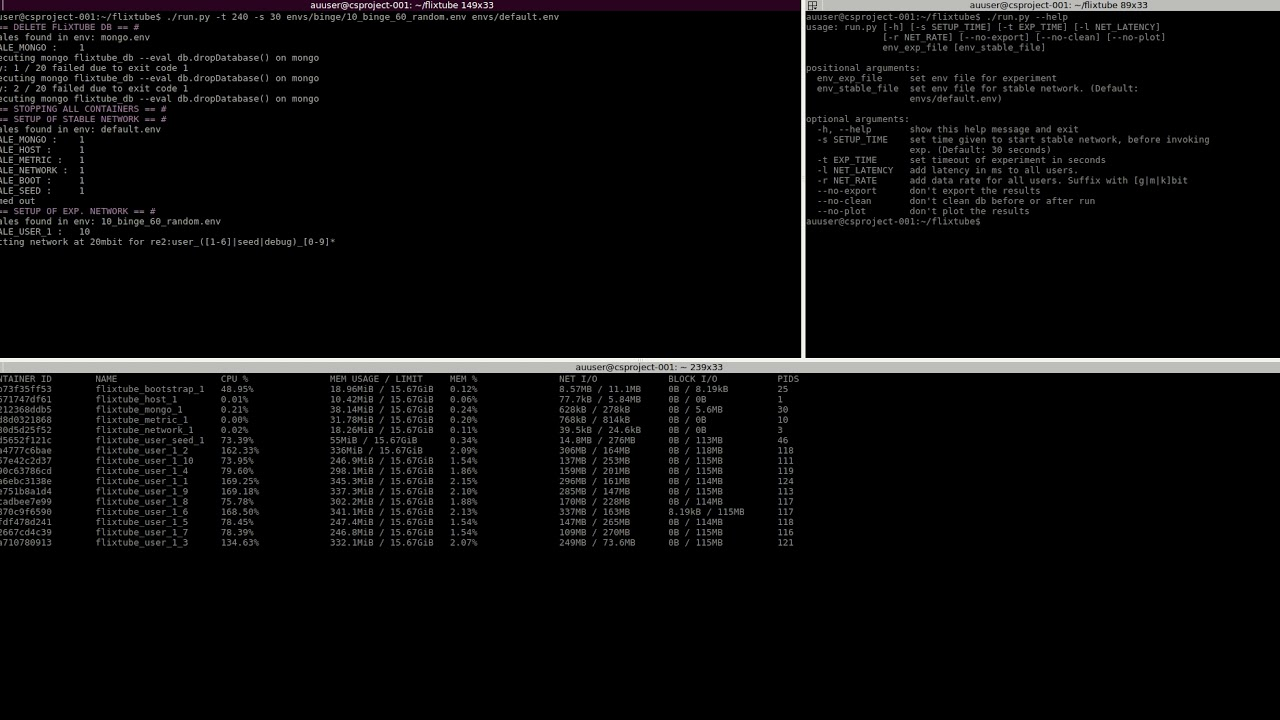
\includegraphics[width=\linewidth]{gfx/demo.jpg}}{https://www.youtube.com/v/_88_Kb7C6FY?rel=0}
\url{https://www.youtube.com/watch?v=_88_Kb7C6FY}

\chapter{Media Presentation Description}
\label{app:mpd}

\lstinputlisting[
    language=MPD,
    caption={[A full \acs{MPD} example.]A full \acs{MPD} example generated by \texttt{MP4Box}. The file have been slightly modified for readability by adding newlines.}
    ]{code/dashed.mpd}

\chapter{Docker Compose files}
\label{app:compose}

\chapter{Collection of Experimental Setups}
\label{app:exp_overviews}
Collection of all named experimental setups and their ID, presented in table overviews from \autoref{cha:evaluation}.

\begin{table}[ht]
    \myfloatalign
    \rptcaption{tab:exp_overview_baseline}
    \colorbox{lightyellow}{
\begin{tabularx}{\textwidth}{lX}
    \toprule
        \tableheadline{Exp. ID} & \tableheadline{Experimental Setup of Network} \\
    \midrule
        \setexpid{B1}    &  1 Binger is introduced to the default stable network. \newline 
                            Network bandwidth is at 20 \acs{MBps}.   \\
%        \dots            & \dots                                     \\
        \setexpid{B5}    &  5 Binges are introduced to the default stable network. \newline 
                            Network bandwidth is at 20 \acs{MBps}.   \\
%        \dots            & \dots                                     \\
        \setexpid{B10}   &  10 Bingers are introduced to the default stable network. \newline 
                            Network bandwidth is at 20 \acs{MBps}.   \\
    \bottomrule
\end{tabularx}}
\end{table}

\begin{table}[ht]
    \myfloatalign
    \rptcaption{tab:exp_overview_leecher}
    \colorbox{lightyellow}{
\begin{tabularx}{\textwidth}{lX}
    \toprule
        \tableheadline{Exp. ID} & \tableheadline{Experimental Setup of Network}     \\
    \midrule
        \setexpid{L1B9}    & 1 Leecher and 9 Binger is introduced to the default stable network over 60 \acs{s}. Network bandwidth is at 20 \acs{MBps}.   \\
        \setexpid{L5B5}    & 5 Leecher and 5 Binger is introduced to the default stable network over 60 \acs{s}. Network bandwidth is at 20 \acs{MBps}.   \\
        \setexpid{L10}     & 10 Leecher is introduced to the default stable network over 60 \acs{s}. Network bandwidth is at 20 \acs{MBps}.   \\
    \bottomrule
\end{tabularx}}
\end{table}

\begin{table}[ht]
    \myfloatalign
    \rptcaption{tab:exp_overview_skipper}
    \colorbox{lightyellow}{
\begin{tabularx}{\textwidth}{lX}
    \toprule
        \tableheadline{Exp. ID} & \tableheadline{Experimental Setup of Network}     \\
    \midrule
        \setexpid{S5B5}    & 
        5 Skipper and 5 Binger is introduced to the default stable network over 60 \acs{s}. \newline 
        Skipper watch time is 3 \acs{s} and skip time 10 \acs{s}.\newline
        Network bandwidth is at 20 \acs{MBps}.   \\
        \setexpid{S5B5-c}    & 
        5 Skipper and 5 Binger is introduced to the default stable network over 60 \acs{s}. \newline 
        Skipper watch time is 1 \acs{s} and skip time 25 \acs{s}.\newline
        Network bandwidth is at 20 \acs{MBps}.   \\
        \setexpid{S10}     & 
        10 Skipper is introduced to the default stable network over 60 \acs{s}.
        Skipper watch time is 3 \acs{s} and skip time 10 \acs{s}.\newline
        Network bandwidth is at 20 \acs{MBps}.   \\
    \bottomrule
\end{tabularx}}
\end{table}

\begin{table}[ht]
    \myfloatalign
    \rptcaption{tab:exp_overview_incognito}
    \colorbox{lightyellow}{
\begin{tabularx}{\textwidth}{lX}
    \toprule
        \tableheadline{Exp. ID} & \tableheadline{Experimental Setup of Network}     \\
    \midrule
        \setexpid{I5B5}    & 
        5 Incognito users and 5 Bingers are introduced to the default stable network over 60 \acs{s}. \newline 
        Network bandwidth is at 20 \acs{MBps}.   \\
        \setexpid{I10}     & 
        10 Incognito users are introduced to the default stable network over 60 \acs{s}. \newline 
        Network bandwidth is at 20 \acs{MBps}.   \\
    \bottomrule
\end{tabularx}}
\end{table}

\begin{table}[ht]
    \myfloatalign
    \rptcaption{tab:exp_overview_mobile}
    \colorbox{lightyellow}{
\begin{tabularx}{\textwidth}{lX}
    \toprule
        \tableheadline{Exp. ID} & \tableheadline{Experimental Setup of Network}     \\
    \midrule
        \setexpid{B10-m1}    & 
        10 Binge is introduced to the default stable network over 60 \acs{s}.
        Network bandwidth is at 5 \acs{MBps}.   \\
        \setexpid{B10-m2}     & 
        10 Binge is introduced to the default stable network over 60 \acs{s}.
        Network bandwidth is at 20 \acs{MBps} with an add latency of 100$\pm$10 \acs{ms}.   \\
        % \setexpid{B10-m3}     & 
        % 10 Binge is introduced to the default stable network over 60 \acs{s}.
        % Network bandwidth is at 5 \acs{MBps} with an add latency of 100 \acs{ms}.   \\
    \bottomrule
\end{tabularx}}
\end{table}


\begin{table}[ht]
    \myfloatalign
    \rptcaption{tab:exp_overview_leaver}
    \colorbox{lightyellow}{
    \begin{tabularx}{\textwidth}{lX}
    \toprule
        \tableheadline{Exp. ID} & \tableheadline{Experimental Setup of Network} \\
    \midrule
        \setexpid{B10-l}  & 10 Bingers are introduced to a stable default network over 60 \acs{s}. Each client will leave the network upon finishing the video. \newline 
        Network bandwidth is at 20 \acs{MBps}.  \\
    \bottomrule
    \end{tabularx}}
\end{table}

\begin{table}[ht]
    \myfloatalign
    \rptcaption{tab:exp_overview_socialness}
    \colorbox{lightyellow}{
    \begin{tabularx}{\textwidth}{lX}
    \toprule
        \tableheadline{Exp. ID} & \tableheadline{Experimental Setup of Network} \\
    \midrule
        \setexpid{B10-s1}  & 10 Binge is introduced to a stable default network over 10 \acs{s}. Network bandwidth is at 20 \acs{MBps}.  \\
        \setexpid{B10-s2}  & 10 Binge is introduced to a stable default network over 180 \acs{s}. Network bandwidth is at 20 \acs{MBps}.  \\
    \bottomrule
    \end{tabularx}}
\end{table}

\begin{table}[ht]
    \myfloatalign
    \rptcaption{tab:exp_overview_segment}
    \colorbox{lightyellow}{
\begin{tabularx}{\textwidth}{lX}
    \toprule
        \tableheadline{Exp. ID} & \tableheadline{Experimental Setup of Network} \\
    \midrule
        \setexpid{B10-v9}   &  
        10 Binge is introduced to the default stable network. The desired video is divided into segments of approximately 9 \acs{s} duration. 
        Network bandwidth is at 20 \acs{MBps}.   \\
    \bottomrule
\end{tabularx}}
\end{table}


\begin{table}[ht]
    \myfloatalign
    \rptcaption{tab:exp_overview_global}
    \colorbox{lightyellow}{
    \begin{tabularx}{\textwidth}{lX}
    \toprule
        \tableheadline{Exp. ID} & \tableheadline{Experimental Setup of Network} \\
    \midrule
        \setexpid{B10-g}  & 10 Bingers having global \ac{IPFS} access are introduced to a stable \textit{near} default network over 60 \acs{s}. \newline The stable network differs by the 1 Seeder having global \ac{IPFS} access and no bootstrap being present.\newline Network bandwidth is at 20 \acs{MBps}.  \\
    \bottomrule
    \end{tabularx}}
\end{table}


\chapter{Experimental Plots}
\label{app:exp_plots}

% FIXME:\begin{figure}[ht]
    \myfloatalign
    \begin{tikzpicture}
    \begin{axis}[
        ybar,
        ymin=0,
        y filter/.code={\pgfmathparse{#1/1024^2}\pgfmathresult},
        xtick=data,
        xticklabels from table={./data/baseline/network_rx_bytes_tx_bytes_hist_b5.csv}{users},
        x tick label style={rotate=60, anchor=east},
        ylabel={Accumulated bandwidth (\acs{MB})},
        legend style={at={(1.05,1)}, anchor=north west,legend columns=1},]
        \addplot table [
            x expr=\coordindex,
            y={rx},
            ]{./data/baseline/network_rx_bytes_tx_bytes_hist_b5.csv};
        \addplot table [x expr=\coordindex, y={tx}]{./data/baseline/network_rx_bytes_tx_bytes_hist_b5.csv};
        \addplot[black, sharp plot, update limits=false]
                coordinates{(-1, 55992320) (11, 55992320)};
        \legend{received,transmitted}
    \end{axis}
    \draw (8,1.75) node {video size};
    \end{tikzpicture}
    \caption[Total bandwidth from \expid{B5}]{Received and transmitted bytes per client, from the baseline experiment (\expid{B5}).
    Download overhead is as large as factor 2.5 as exemplified by \textit{5:BINGER} receiving 163 \ac{MB} while asking for a 56 \acs{MB} video.}
    \label{bar:baseline_network_hist_b5}
\end{figure}


%%% Local Variables:
%%% mode: latex
%%% TeX-master: "../ClassicThesis"
%%% End:
